\documentclass[12pt]{article}                   % Začátek dokumentu
\usepackage{../../MFFStyle}                     % Import stylu

\begin{document}

\begin{priklad}[A]
    Označme $F=C^∞\(®R^3\)$ prostor hladkých funkcí a $©F^3$ prostor vektorových polí na $®R^3$. Ukažte, že následující posloupnost diferenciálních operátorů tvoří komplex, tj. že složení dvou po sobě následujících operátorů je triviální.
    $$ ©F \overset{\grad}{\longrightarrow} ©F^3 \overset{\rot}{\longrightarrow} ©F^3 \overset{\Div}{\longrightarrow} ©F $$

    \begin{dukazin}[Z definic $\rot \circ \grad$]
        $$ \forall F \in ©F: \rot \circ \grad F = $$
        $$ = \(\frac{\partial \(\grad F\)_z}{\partial y} - \frac{\partial \(\grad F\)_y}{\partial z}; \frac{\partial \(\grad F\)_x}{\partial z} - \frac{\partial \(\grad F\)_z}{\partial x}; \frac{\partial \(\grad F\)_y}{\partial x} - \frac{\partial \(\grad F\)_x}{\partial y}\)^T = $$ 
        $$ = \(\frac{\partial}{\partial y}\frac{\partial F}{\partial z} - \frac{\partial}{\partial z}\frac{\partial F}{\partial y}; \frac{\partial}{\partial z}\frac{\partial F}{\partial x} - \frac{\partial}{\partial x}\frac{\partial F}{\partial z}; \frac{\partial}{\partial x}\frac{\partial F}{\partial y} - \frac{\partial}{\partial y}\frac{\partial F}{\partial x}\)^T = (0, 0, 0)^T, $$ 
        Jelikož z matematické analýzy víme, že nezáleží na pořadí parciálního derivování.
    \end{dukazin}

    \begin{dukazin}[Z definic $\Div \circ \rot$]
        $$ \forall \vec{F} \in ©F^3: \Div \circ \rot \vec{F} = $$
        $$ = \frac{\partial \(\rot\vec{F}\)_x}{\partial x} + \frac{\partial \(\rot\vec{F}\)_y}{\partial y} + \frac{\partial \(\rot\vec{F}\)_z}{\partial z} = $$
        $$ = \frac{\partial \(\frac{\partial F_z}{\partial y} - \frac{\partial F_y}{\partial z}\)}{\partial x} + \frac{\partial \(\frac{\partial F_x}{\partial z} - \frac{\partial F_z}{\partial x}\)}{\partial y} + \frac{\partial \(\frac{\partial F_y}{\partial x} - \frac{\partial F_x}{\partial y}\)}{\partial z} = $$
        $$ = \frac{\partial^2 F_z}{\partial y\partial x} - \frac{\partial^2 F_y}{\partial z \partial x} + \frac{\partial^2 F_x}{\partial z \partial y} - \frac{\partial^2 F_z}{\partial x \partial y} + \frac{\partial^2 F_y}{\partial x \partial z} - \frac{\partial^2 F_x}{\partial y \partial z} = 0 $$
        $$  $$ 
        Ze stejného důvodu jako výše.
    \end{dukazin}
\end{priklad}

\pagebreak

\begin{priklad}[B]
    Ukažte, že následující diagram je komutativní diagram, tj. že složení operátorů spojujících libovolné dva uzly diagramu nezávisí na volbě cesty mezi příslušnými dvěma uzly.
    
    \ \hfill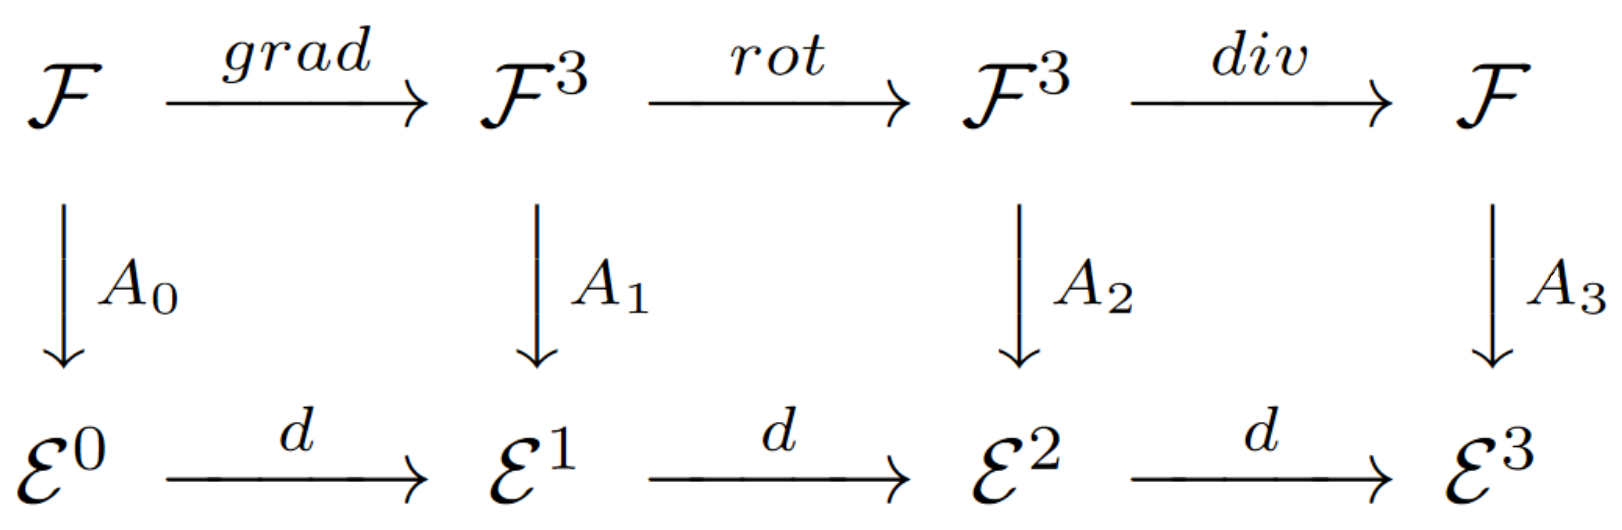
\includegraphics[scale=0.3]{diagram.png}\hfill\ 
    $$ A_0 = \id, \quad A_1(\vec{F}) = F_x\,dx + F_y\,dy + F_z\,dz, \quad A_2(\vec{F}) = F_x\,dy\wedge dz + F_y\,dz\wedge dx + F_z\,dx\wedge dy, $$
    $$ A_3(F) = F\, dx \wedge dy \wedge dz. $$ 

    \begin{dukazin}[Z definic $d \circ A_0 = A_1 \circ \grad$]
        $$ \forall F \in ©F: (d \circ A_0)(F) = dF = \frac{\partial F}{\partial x}\,dx + \frac{\partial F}{\partial y}\,dy + \frac{\partial F}{\partial z}\,dz = $$
        $$ = (\grad F)_x\,dx + (\grad F)_y\,dy + (\grad F)_z\,dz = A_1 \circ \grad F. $$
    \end{dukazin}

    \begin{dukazin}[Z definic $d \circ A_1 = A_2 \circ \rot$]
        $$ \forall \vec{F} \in ©F^3: (d \circ A_1)(\vec{F}) = d(F_x\,dx + F_y\,dy + F_z\,dz) = $$
        $$ = \(\frac{\partial F_x}{\partial x}dx + \frac{\partial F_x}{\partial y}dy + \frac{\partial F_x}{\partial z}dz\)\wedge dx + $$
        $$ + \(\frac{\partial F_y}{\partial y}dx + \frac{\partial F_y}{\partial y}dy + \frac{\partial F_y}{\partial z}dz\)\wedge dy + $$
        $$ + \(\frac{\partial F_z}{\partial x}dx + \frac{\partial F_z}{\partial y}dy + \frac{\partial F_z}{\partial z}dz\)\wedge dz = $$
        $$ 0 + \(\frac{\partial F_y}{\partial x}-\frac{\partial F_x}{\partial y}\)dx \wedge dy + \(\frac{\partial F_x}{\partial z}-\frac{\partial F_z}{\partial x}\)dz \wedge dx + 0 + \(\frac{\partial F_z}{\partial y}-\frac{\partial F_y}{\partial z}\)dy \wedge dz + 0 = $$
        $$ = (\rot\vec{F})_x\,dy \wedge dz + (\rot\vec{F})_y\,dz \wedge dx + (\rot\vec{F})_z\,dx \wedge dy = A_2 \circ \rot \vec{F}. $$ 
    \end{dukazin}

    \begin{dukazin}[Z definic $d \circ A_2 = A_3 \circ \Div$]
        $$ \forall \vec{F} \in ©F^3: (d \circ A_2)(\vec{F}) = d(F_x\,dy\wedge dz + F_y\,dz \wedge dx + F_z\,dx \wedge dy) = $$
        $$ = \(\frac{\partial F_x}{\partial x}dx + \frac{\partial F_x}{\partial y}dy + \frac{\partial F_x}{\partial z}dz\)\wedge dy \wedge dz + $$
        $$ + \(\frac{\partial F_y}{\partial y}dx + \frac{\partial F_y}{\partial y}dy + \frac{\partial F_y}{\partial z}dz\)\wedge dz \wedge dx + $$
        $$ + \(\frac{\partial F_z}{\partial x}dx + \frac{\partial F_z}{\partial y}dy + \frac{\partial F_z}{\partial z}dz\)\wedge dx \wedge dy = $$
        $$ \(\frac{\partial F_x}{\partial x} + \frac{\partial F_y}{\partial y} + \frac{\partial F_z}{\partial z} \)dx \wedge dy \wedge dz + 6·0 = \Div\vec{F}\,dx \wedge dy \wedge dz = A_3 \circ \Div \vec{F}. $$ 
    \end{dukazin}

    \begin{dukazin}[Zbylé]
        Komutativita složení více (>2) operátorů vyplývá z předchozích.
    \end{dukazin}
\end{priklad}

\end{document}
